\documentclass[11pt]{article}
\usepackage{geometry}                % See geometry.pdf to learn the layout options. There are lots.
\geometry{letterpaper}                   % ... or a4paper or a5paper or ... 
%\geometry{landscape}                % Activate for for rotated page geometry
\usepackage[parfill]{parskip}    % Activate to begin paragraphs with an empty line rather than an indent
\usepackage{graphicx}
\usepackage{amssymb}
\usepackage{natbib}
\usepackage{epstopdf}

\usepackage[colorlinks=true, pdfstartview=FitV, linkcolor=blue, 
            citecolor=blue, urlcolor=blue]{hyperref}

\DeclareGraphicsRule{.tif}{png}{.png}{`convert #1 `dirname #1`/`basename #1 .tif`.png}

\title{Evaluating Bayesian Networks as a Tool for Reasoning with Evidence using Agent-Based Simulations}
\author{Ludi van Leeuwen}
\date{}                                                   % Activate to display a given date or no date

\begin{document}
\maketitle
%\section{}
%\subsection{}


\section{Introduction}
When we find evidence for a hypothesis that we have held in the back of our minds, our belief in that hypothesis increases. This is the essence of reasoning with evidence. Our goal in reasoning with evidence is to find a method that will lead us to believe as many true hypotheses as we can, given the evidence that we have.

However, the relationship between evidence and hypotheses is elusive. How can we be sure that some evidence supports some hypothesis? Even if we know that it does, how can we express how strong the piece of evidence is? Some evidence is very weak, and only after a tedious process of ruling out other factors and careful investigation and collection of other pieces of evidence, we can come to a conclusion about a hypothesis. On the other hand, some evidence is so strong that it leaves no room for doubt.

We can consider three main approaches for reasoning about hypotheses using evidence within the domain of AI and Law \citep{diBelloVerheij2018}: an argumentative, a scenario-based, and a probabilistic approach. One subfield of the probabilistic approach is the use of Bayesian Networks. Bayesian Networks can make explicit how our beliefs about events should change given that we find certain pieces of evidence for them. This idea of correctly updating on new information make BNs an interesting tool in the courtroom. A Bayesian Network might make transparent how reasoners should update their beliefs based on the evidence, which might increase transparency and fairness. In the ideal case, a Bayesian Network might stop a judge from making a reasoning error.

However, creating and using BNs is far from straightforward for both the builder and the interpreter. From \citet{deKoeijer2020}: it is complex, time-consuming, hard to explain, and, the ``repeatability [...] leaves much to be desired. Node definitions and model structures are often directed by personal habits, resulting in different models for the same problem, depending on the expert''. This subjectivity is pervasive throughout the Bayesian Network: the events selected, arcs drawn, and numbers elicited are subjective and seem empirically untestable in the data-poor environment of AI and law. These problems might be mitigated in part by evaluation criteria. 

These evaluation criteria, however, do do not always sufficiently safeguard against an incorrect network, which is a network that predict the `wrong' outcome based on some set of evidence. One example of this is seen in Figure~\ref{love}, which is a network taken from \citet{vanLeeuwen2019}. This network is unfairly biased towards the scenario that the suspect is guilty. In the original paper, we entered the evidence that was found during the trial, and the response of the network seemed sensible. However, in that same network, we are now entering a different evidence: there is no body, no signs of violence, no car with bloodstains, no evidence of existing conflict. The only evidence that the prosecution has, are some phone calls, and  testimony of the suspect about amnesia that does not match medical reality. The outcome of the network is that the suspect is guilty (scn1 is `yes'). But the evidence that is entered into this network, would not reasonably support this conclusion. No reasonable arguer would argue that this state of evidence is sufficient for a guilty verdict.

\begin{figure}[htbp]
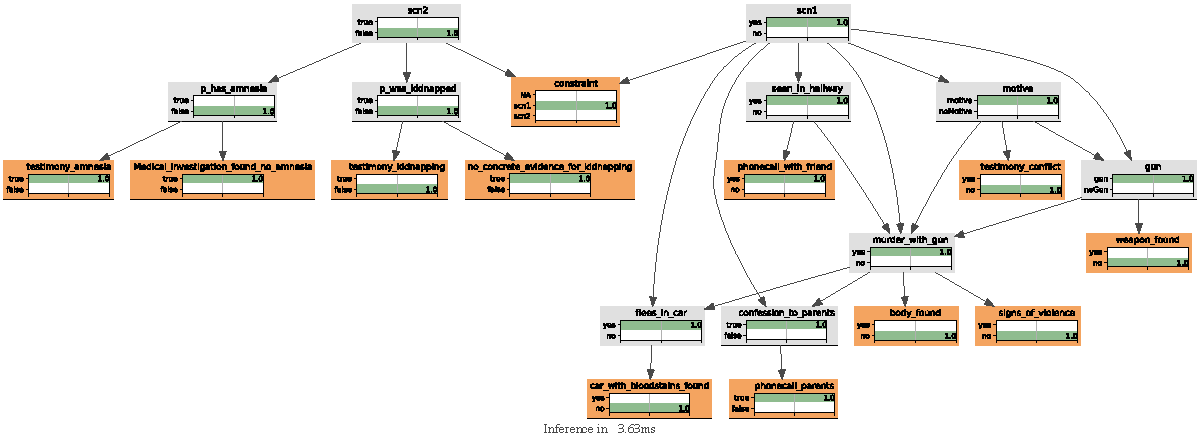
\includegraphics[width=\linewidth]{images/oldnetwork.pdf}
\caption{Example of subjective probability estimation resulting in a guilty verdict for insufficient evidence}
\label{love}
\end{figure}%


The cause of the bias of this BN towards the guilty verdict is due to the modeller's inability to rationally consider all possible evidence states. The aim of this project is to define a method for the modeller to evaluate the BN over all possible evidence states, by grounding the BN in an agent-simulation of a crime. We can model crime cases using simulations to a level of realism we desire, measure the frequencies of events that emerge out of this simulation by running the simulation multiple times. In the agent-based system, we have full control over and full knowledge of the world that we are reasoning about, hence we can create a grounding that can be used to evaluate the BN. We can test whether our method of evaluating all possible evidence states works by comparing the predicted output of the BN with the frequency information about the output from the simulation. Then, we will discuss whether it is plausible that this method of evaluation generalises to real life\footnote{The simulation can be interacted with at \url{https://shielded-journey-34533.herokuapp.com} \\ Code for this project can be found at \url{https://github.com/aludi/simulationTest}}.

\newpage

\bibliographystyle{apalike}
\bibliography{masterThesisCitations}

\end{document}  